\documentclass[12pt,a4paper]{article}

%% ── Packages ───────────────────────────────────────────────────────────────
\usepackage[T1]{fontenc}
\usepackage[utf8]{inputenc}
\usepackage{lmodern}
\usepackage[margin=2.5cm]{geometry}
\usepackage{microtype}
\usepackage{setspace}
\onehalfspacing

\usepackage{amsmath,amssymb}
\usepackage{graphicx}
\usepackage{xcolor}
\usepackage{booktabs}
\usepackage{array}
\usepackage{tabularx}
\usepackage{longtable}
\usepackage{multirow}
\usepackage{makecell}
\usepackage{hyperref}
\usepackage{url}
\usepackage{natbib}
\usepackage{authblk}
\usepackage{abstract}
\usepackage{titlesec}
\usepackage{enumitem}
\usepackage{caption}
\usepackage{subcaption}
\usepackage{listings}
\usepackage{float}

%% TikZ for pipeline diagrams
\usepackage{tikz}
\usetikzlibrary{arrows.meta, shapes.geometric, shapes.misc, fit,
                positioning, calc, backgrounds, decorations.pathreplacing}

%% ── Hyperref setup ─────────────────────────────────────────────────────────
\hypersetup{
  colorlinks  = true,
  linkcolor   = blue!60!black,
  citecolor   = green!40!black,
  urlcolor    = blue!60!black,
  pdfauthor   = {VarForge Authors},
  pdftitle    = {VarForge: A Comprehensive Rust-Based Framework for Synthetic Cancer Sequencing Data Generation},
}

%% ── Section formatting ─────────────────────────────────────────────────────
\titleformat{\section}{\large\bfseries}{\thesection.}{0.5em}{}
\titleformat{\subsection}{\normalsize\bfseries}{\thesubsection.}{0.5em}{}
\titleformat{\subsubsection}{\normalsize\itshape}{\thesubsubsection.}{0.5em}{}

%% ── Listing style (YAML examples) ──────────────────────────────────────────
\definecolor{yamlkeycolor}{HTML}{0000AA}
\definecolor{yamlvalcolor}{HTML}{007700}
\definecolor{yamlcomcolor}{HTML}{888888}
\definecolor{lstbg}{HTML}{F8F8F8}
\lstdefinelanguage{yaml}{
  keywords={true,false,null,yes,no},
  keywordstyle=\color{yamlkeycolor}\bfseries,
  comment=[l]{\#},
  commentstyle=\color{yamlcomcolor}\itshape,
  stringstyle=\color{yamlvalcolor},
  sensitive=false,
  morestring=[b]',
  morestring=[b]",
}
\lstset{
  basicstyle=\footnotesize\ttfamily,
  backgroundcolor=\color{lstbg},
  frame=single,
  framerule=0.4pt,
  breaklines=true,
  showstringspaces=false,
}

%% ── Custom commands ─────────────────────────────────────────────────────────
\newcommand{\todo}[1]{\textbf{\textcolor{red}{[TODO: #1]}}}
\newcommand{\varforge}{\textsc{VarForge}}
\newcommand{\bamsurgeon}{\textsc{BAMSurgeon}}
\newcommand{\eg}{\textit{e.g.},\xspace}
\newcommand{\ie}{\textit{i.e.},\xspace}

%% ── TikZ colour palette ────────────────────────────────────────────────────
\definecolor{pipeblue}{HTML}{2E86AB}
\definecolor{pipegreen}{HTML}{27AE60}
\definecolor{pipeorange}{HTML}{E67E22}
\definecolor{pipegray}{HTML}{7F8C8D}
\definecolor{pipeyellow}{HTML}{F39C12}
\definecolor{pipered}{HTML}{C0392B}
\definecolor{pipelightblue}{HTML}{AED6F1}
\definecolor{pipelightgreen}{HTML}{A9DFBF}

%%═══════════════════════════════════════════════════════════════════════════
\begin{document}

%%────────────────────────────────────────────────────────────────────────────
%%  Title block
%%────────────────────────────────────────────────────────────────────────────
\title{\varforge{}: A Comprehensive Rust-Based Framework for Synthetic\\
       Cancer Sequencing Data Generation}

\author[1]{Authors Redacted for Review}
\affil[1]{Institution}

\date{}
\maketitle
\thispagestyle{empty}

%%────────────────────────────────────────────────────────────────────────────
%%  Abstract
%%────────────────────────────────────────────────────────────────────────────
\begin{abstract}
\noindent
Accurate benchmarking of cancer genomics pipelines demands synthetic sequencing
datasets with precisely known ground truth.  However, no single existing tool
integrates de-novo read generation, somatic variant spike-in, tumour purity and
clonal-architecture modelling, unique molecular identifier~(UMI) and duplex
sequencing simulation, cell-free DNA~(cfDNA) fragmentation, and library
artefact injection into a unified, high-performance framework.  Current
practice chains three to five heterogeneous tools---each with separate
dependencies, file-format assumptions, and documentation quality---introducing
integration fragility and hours of manual setup.

We present \varforge{}, a single-binary, pure-Rust framework that addresses
every one of these gaps in a single, composable tool driven by a
human-readable YAML configuration.  \varforge{} is the first simulator to
provide genome-wide UMI and duplex sequencing simulation, the first dedicated
in-silico cfDNA fragmentation engine with somatic variant spike-in capability,
and the first to combine stochastic variant allele frequency~(VAF) sampling,
clonal-tree tumour models, copy number variant support, FFPE and oxidative
artefacts, and GC-bias correction in one integrated system.  A parallel,
streaming architecture built on the Rayon work-stealing scheduler enables
throughput that is substantially faster than existing Python- and
Java-based alternatives, with a peak memory footprint that scales with thread
count rather than dataset size.

Benchmarking on a 6-core laptop-class system (AMD Ryzen 5 7640HS,
12\,GiB RAM, Rust~1.94) demonstrates sustained throughput of
$\sim$4.0\,Gbp/min ($\sim$13{,}400 read pairs/sec) for 30$\times$
whole-genome simulation on a 10\,MB synthetic reference using 12
threads, with a wall-clock ceiling of $\sim$12.4 hours projected for
30$\times$ full-human-genome simulation.  On compute-bound panel
workloads the throughput rises to $\sim$8.4\,Gbp/min ($\sim$28{,}000
read pairs/sec).  Runtime overhead for variant injection, GC-bias
correction, FFPE/oxoG artefacts, and cfDNA fragment modelling ranges
from negligible ($<$3\%) to 16\%, while UMI simulation adds 64\% due
to PCR family genealogy tracking.  These figures compare favourably
with existing Python-based alternatives whose interpreter overhead
substantially limits WGS-scale throughput.
\varforge{} is freely available as an open-source MIT-licensed tool at
\url{https://github.com/varforge/varforge}.
\end{abstract}

\noindent\textbf{Keywords:} synthetic sequencing data; cancer genomics;
variant simulation; UMI; duplex sequencing; cell-free DNA; bioinformatics
benchmarking; Rust

\newpage
\tableofcontents
\newpage

%%────────────────────────────────────────────────────────────────────────────
%%  1. Introduction
%%────────────────────────────────────────────────────────────────────────────
\section{Introduction}
\label{sec:intro}

High-throughput sequencing has transformed cancer research, enabling
the systematic identification of somatic mutations, copy number
alterations, structural rearrangements, and tumour evolutionary
dynamics at single-base resolution.  The downstream analytical tools
that process this data---variant callers, UMI-deduplication pipelines,
copy number estimators, and liquid-biopsy algorithms---must be
rigorously benchmarked before clinical or research deployment.  Robust
benchmarking requires sequencing datasets in which the complete ground
truth is known: every injected variant, its exact allele frequency, its
clone of origin, and its interaction with platform artefacts.  Real patient
data cannot satisfy this requirement; even the best orthogonal validation
strategies leave uncertainty in the ground truth.  Synthetic sequencing
simulation therefore occupies an indispensable role in pipeline
development, method comparison, and reproducibility assurance.

Cancer sequencing introduces simulation challenges that generic read
simulators were never designed to address.  A realistic cancer dataset
must capture~(i)~the mixture of tumour and normal cells, parametrised by
purity and clonal-architecture; ~(ii)~allele-frequency heterogeneity
arising from sub-clonal evolution; ~(iii)~copy number alterations that
alter both coverage depth and the effective variant allele frequency
at affected loci; ~(iv)~a spectrum of variant types ranging from single
nucleotide variants~(SNVs) and small indels through multi-nucleotide
variants~(MNVs), structural variants~(SVs), and whole-arm copy number
events; ~(v)~library preparation artefacts such as FFPE-associated C$>$T
deamination and oxidative 8-oxoG damage; and ~(vi)~cfDNA fragmentation
profiles when the specimen is derived from liquid biopsy.

Despite a rich ecosystem of individual tools, no single framework covers
this entire space.  Existing simulators fall into at least three
non-overlapping categories: BAM-editing tools that spike variants into
pre-existing reads (\eg \bamsurgeon{}~\citep{ewing2015bamsurgeon},
SomatoSim~\citep{kuhnemund2017somatomsim}); de-novo read generators
that produce FASTQ output from a reference genome (\eg
ART~\citep{huang2012art}, NEAT~\citep{stephens2016neat},
ReSeq~\citep{schmeing2021reseq}); and cancer-evolution simulators that
model clonal dynamics but delegate read generation to external tools
(\eg PSiTE~\citep{psyte2020psite}, VarSim~\citep{mu2015varsim}).
Benchmarking a single analysis pipeline therefore requires assembling
and orchestrating a bespoke chain of tools, each with its own
installation requirements, intermediate file formats, and stochastic
seeding conventions.

Two critical capabilities are entirely absent from the existing
landscape.  First, no genome-wide simulator for UMI-tagged or duplex
sequencing data exists.  UMI-tools~\citep{smith2017umitools} offers
single-locus amplification simulation only, and the Kennedy Lab duplex
pipeline bundles basic test data generation rather than a configurable
simulation framework.  As a result, tools such as fgbio~\citep{fgbio},
UMI-tools, and HUMID rely on circular benchmarking---using the same
tool both to annotate and to evaluate synthetic data---or on manually
constructed ad-hoc datasets.  Second, no dedicated in-silico cfDNA
simulator exists that combines nucleosomal fragmentation with somatic
variant spike-in capability.  ichorCNA~\citep{adalsteinsson2017ichorcna}
and DELFI~\citep{cristiano2019delfi} are validated against real patient
samples; the absence of a configurable in-silico cfDNA generator
prevents the comprehensive sensitivity and specificity benchmarking
these tools require.

A further methodological limitation pervades the BAM-editing tools:
deterministic variant spike-in.  When \bamsurgeon{} injects a variant at
10\% VAF into a 30$\times$ BAM, it modifies exactly three reads.  Real
sequencing is a stochastic sampling process; the observed alt-read count
follows a binomial distribution around the expected VAF, not a fixed
value.  Benchmarks built on deterministic spike-in overestimate the
performance of downstream callers by presenting them with unnaturally
clean data~\citep{osullivan2023stochasticsim}.

We present \varforge{}, a Rust-based simulation framework that addresses
all of these gaps simultaneously within a single binary.  The
contributions of this work are:

\begin{enumerate}[leftmargin=*, label=(\roman*)]
  \item A unified cancer sequencing simulation pipeline covering de-novo
        read generation, somatic variant injection, tumour purity/clonal
        architecture, copy number alteration, UMI and duplex sequencing,
        cfDNA fragmentation, and library artefacts---all driven by a
        single YAML configuration.
  \item The first genome-wide simulator for UMI-tagged and duplex
        sequencing data, enabling principled benchmarking of consensus-
        calling tools such as fgbio and UMI-tools.
  \item The first dedicated in-silico cfDNA fragment generator that
        incorporates a nucleosomal mixture model with 10\,bp periodicity
        and supports somatic variant spike-in, enabling sensitivity
        benchmarking for liquid-biopsy tools.
  \item Stochastic VAF sampling via per-read Bernoulli trials, eliminating
        the systematic optimism introduced by deterministic spike-in tools.
  \item A streaming, parallel implementation in Rust achieving substantially
        higher throughput than existing Python- and Java-based tools,
        without sacrificing reproducibility.
\end{enumerate}

The remainder of this paper is organised as follows.
Section~\ref{sec:background} reviews related tools and characterises the
gaps that motivated \varforge{}.  Section~\ref{sec:methods} describes
the architecture and algorithmic details of each simulation component.
Section~\ref{sec:results} presents benchmarking results (\textit{results
to be added after benchmarking}).  Section~\ref{sec:discussion} discusses
implications, limitations, and future directions.
Section~\ref{sec:conclusion} concludes.

%%────────────────────────────────────────────────────────────────────────────
%%  2. Background and Related Work
%%────────────────────────────────────────────────────────────────────────────
\section{Background and Related Work}
\label{sec:background}

\subsection{Somatic Variant Simulation via BAM Editing}
\label{sec:bg:bam-editing}

The dominant approach to generating cancer benchmark data has been to
inject synthetic variants into an existing ``normal'' BAM file, replacing
a fraction of real reads at each target locus with reads carrying the
desired alternate allele.

\bamsurgeon{}~\citep{ewing2015bamsurgeon} established this paradigm and
became the de-facto standard through its use in the ICGC-TCGA DREAM
Somatic Mutation Calling Challenge~\citep{ewing2015bamsurgeon}.  It
supports SNVs, small indels, and structural variants (SVs) and interfaces
with multiple aligners for local re-mapping of modified reads.  Despite
its status, \bamsurgeon{} has well-known limitations: it requires a
high-coverage input BAM ($\geq 30\times$) and is computationally slow,
taking on the order of 4--5 seconds per variant, making whole-genome
benchmarking with tens of thousands of mutations impractical.  More
critically, \bamsurgeon{} applies a deterministic spike-in: a target of
10\% VAF at 30$\times$ depth always results in exactly three alt reads,
systematically overestimating the performance of variant callers on real
data.  \bamsurgeon{} has no support for UMI barcodes, cfDNA fragmentation,
or library artefact simulation, and as of~2022 is in maintenance mode.

SomatoSim~\citep{kuhnemund2017somatomsim} addresses some usability
concerns, offering precise control over variant positions and a fast
runtime ($\sim$44 seconds for runs that require $\sim$56 minutes with
\bamsurgeon{}).  However, SomatoSim is limited to SNVs, targets only
exome or targeted sequencing data, and applies the same deterministic
spike-in logic.

stochasticSim~\citep{osullivan2023stochasticsim} represents a meaningful
methodological advance: it builds haplotype-resolved personalised tumour
genomes from 1000~Genomes phased data, and it models stochastic sampling
error so that observed alt-read counts follow a binomial distribution
around the expected VAF.  It also includes FFPE C$>$T deamination and
8-oxoG artefacts---the only existing tool to do so.  However,
stochasticSim is limited to SNVs, operates at exome scale, and does not
support UMI barcodes, cfDNA fragmentation, or de-novo read generation.

\subsection{De-Novo Read Simulators}
\label{sec:bg:read-sim}

ART~\citep{huang2012art} generates synthetic Illumina, 454, and SOLiD
reads using empirical, position-dependent quality score profiles derived
from large real datasets.  It was one of the first simulators to match
observed error-rate distributions closely, and with over 3{,}500
citations it remains the most widely used read simulator.  The original
implementation is single-threaded, last released in~2016, and lacks any
variant injection, tumour modelling, UMI support, or cfDNA simulation.
An actively maintained community reimplementation, \texttt{art\_modern},
adds MPI parallelism and BAM output.

NEAT~\citep{stephens2016neat} (NExt-generation sequencing Analysis
Toolkit) learns mutation and error models from real datasets and supports
VCF-guided variant injection of SNVs, indels, and inversions.  The v4
series adds multi-threading and maintains active development.  NEAT is
implemented in Python, which limits throughput at WGS scale; it has no
cancer tumour model, UMI/duplex simulation, cfDNA fragmentation, or
artefact injection.

ReSeq~\citep{schmeing2021reseq} is the most fidelity-oriented Illumina
simulator available.  It learns systematic errors, fragment-level
coverage variation, GC bias, and PCR duplicate rates from a real BAM
file, then reproduces these patterns during simulation.  ReSeq sets
the standard for read-level realism but does not support variant
injection, cancer or tumour modelling, UMI barcodes, or cfDNA
fragmentation.

DWGSIM is a lightweight C-based simulator suitable for rapid generation
of reads with configurable uniform or position-dependent error rates; it
lacks empirical quality profiles and cancer-specific features.  wgsim is
even more minimal---a single C source file with no dependencies---and
is primarily used for quick smoke tests.  NGSNGS~\citep{ngsngs2023}
offers a multi-threaded design and is faster than many alternatives but
similarly lacks cancer, UMI, and cfDNA capabilities.

\subsection{Cancer Evolution Simulators}
\label{sec:bg:cancer-evo}

VarSim~\citep{mu2015varsim} provides an end-to-end framework: it
synthesises diploid genomes with germline and somatic mutations drawn
from realistic variant databases, and automates simulation and validation
by invoking external read simulators (ART or DWGSIM) as backends.
VarSim supports SNVs, indels, and large SVs, and can generate
tumour-normal pairs.  However, it depends on a complex Java\,+\,Python
stack, its last release was in~2020, and it has no UMI, cfDNA, or
artefact simulation.

PSiTE~\citep{psyte2020psite} models tumour evolution guided by
phylogenetic trees, supporting both bulk and single-cell modes.  It
generates clone genomes with cumulative somatic events and calls
external read simulators to produce FASTQ/BAM output.  The multi-module
pipeline architecture makes integration fragile and requires external
toolchain management.

MOV\&RSim~\citep{movsim2025} (published 2025) was motivated by the
observation that none of the nine existing somatic simulators its authors
evaluated provided complete control over both biological and technical
simulation parameters.  It introduces cancer-type-specific presets for
21 cancer types and is distributed as a Docker container.  As a recent
tool it has a small user base, and it does not support UMI/duplex
sequencing or cfDNA simulation.

GENOMICON-Seq~\citep{genomiconseq2025} (published 2025) models the full
library preparation pipeline including PCR amplification errors,
probe-capture enrichment, and Illumina sequencing biases.  It simulates
APOBEC3 edits and COSMIC mutational signatures, and tracks ground truth
through the entire pipeline.  However, it lacks UMI/duplex simulation,
cfDNA fragmentation modelling, and clonal architecture support.

\subsection{UMI and Duplex Sequencing: A Gap}
\label{sec:bg:umi-gap}

Duplex sequencing~\citep{schmitt2012duplex} achieves error rates of
$10^{-7}$--$10^{-10}$ per base by independently sequencing both strands
of each original DNA molecule and requiring agreement between the two
strand-specific consensus sequences.  It is increasingly deployed for
ultra-low VAF detection in liquid biopsy, minimal residual disease
(MRD) monitoring, and mutagenesis studies.  The downstream analysis
tools---fgbio~\citep{fgbio}, UMI-tools~\citep{smith2017umitools},
HUMID, and UMIErrorCorrect---require benchmark datasets with known
per-read UMI sequences, known PCR family assignments, and known true
mutations versus sequencing artefacts.

No general-purpose genome-wide UMI or duplex sequencing simulator
exists.  UMI-tools provides single-locus amplification simulation only.
The Kennedy Lab pipeline bundles test data that cannot be reconfigured
for different loci, family sizes, or duplex architectures.  The result
is that UMI analysis tools are benchmarked through circular evaluation
(the same tool both generates and evaluates the synthetic UMI data) or
with manually constructed datasets of limited scope.  \varforge{} is
designed to fill this gap.

\subsection{Cell-Free DNA Simulation: A Gap}
\label{sec:bg:cfdna-gap}

Cell-free DNA in plasma has a characteristic fragmentation pattern
determined by nucleosomal protection: the predominant fragment class
spans a single nucleosome ($\sim$167\,bp), with subordinate populations
at di-nucleosomal ($\sim$334\,bp) and tri-nucleosomal ($\sim$500\,bp)
lengths, and a 10\,bp periodicity below 167\,bp reflecting the helical
pitch of DNA wound around the histone octamer~\citep{snyder2016cfdna_nucleosome}.
Tumour-derived ctDNA fragments are shorter than normal cfDNA, enriched
below 167\,bp, with a peak near 143--147\,bp~\citep{lo2010cfdna}.
These fragmentation patterns are exploited by fragmentation analysis
tools such as DELFI~\citep{cristiano2019delfi} and by copy number
estimators such as ichorCNA~\citep{adalsteinsson2017ichorcna}.

Fragmentstein~\citep{fragmentstein2024} converts tabulated fragment
coordinates into paired-end BAM files but does not generate fragments
de novo.  FinaleToolkit analyses real cfDNA patterns but does not simulate
them.  The shendurelab/cfDNA codebase extracts distributions from real
data and generates aligned reads but provides no somatic variant spike-in
capability and is research-grade code not intended as a general tool.
No production-ready in-silico cfDNA simulator with variant support
therefore exists.  \varforge{} addresses this by implementing a
parametric nucleosomal mixture model directly within its fragment
generation engine.

\subsection{Library Artefact Modelling}
\label{sec:bg:artefacts}

FFPE (formalin-fixed, paraffin-embedded) tissue fixation causes
cytosine deamination that manifests as C$>$T transitions (G$>$A on the
opposite strand), which mimic somatic SNVs and are a major source of
false positives in FFPE-derived tumour sequencing.  Oxidative damage
at 8-oxoguanine sites produces G$>$T (C$>$A) transversions with a
characteristic strand bias.  Only stochasticSim~\citep{osullivan2023stochasticsim}
models both artefact types, but it cannot be combined with de-novo read
generation, UMI simulation, or cfDNA fragmentation.  ReSeq~\citep{schmeing2021reseq}
models GC bias and PCR duplicates using negative-binomial rates learned
from real data, but does not model FFPE or oxidative damage.
GENOMICON-Seq~\citep{genomiconseq2025} models PCR amplification errors
through the full amplification chain but does not model FFPE or oxidative
artefacts.  No single tool integrates all four artefact classes
(FFPE deamination, oxidative damage, PCR duplicates, PCR errors) with
the rest of the simulation pipeline.

%%────────────────────────────────────────────────────────────────────────────
%%  3. Methods / Architecture
%%────────────────────────────────────────────────────────────────────────────
\section{Methods and Architecture}
\label{sec:methods}

\subsection{System Overview}
\label{sec:methods:overview}

Figure~\ref{fig:pipeline} illustrates the \varforge{} pipeline.  At
the highest level, a validated YAML configuration drives all simulation
parameters.  The reference genome is indexed and memory-mapped at startup;
variant definitions are read from an optional VCF file or generated
stochastically from user-specified count, type fractions, and VAF ranges.
The genome is then partitioned into non-overlapping regions (by default,
one per chromosome), and each region is processed independently by a
worker thread.  Within each worker, four logical stages execute in
sequence: fragment sampling, variant spike-in, quality score assignment,
and artefact injection.  Workers send completed region batches through a bounded
\texttt{crossbeam-channel} to a dedicated writer thread that writes
the final FASTQ or BAM output.  A truth VCF
recording every injected variant, its achieved VAF, and its clone of
origin is written in parallel with the primary output.

\begin{figure}[H]
\centering
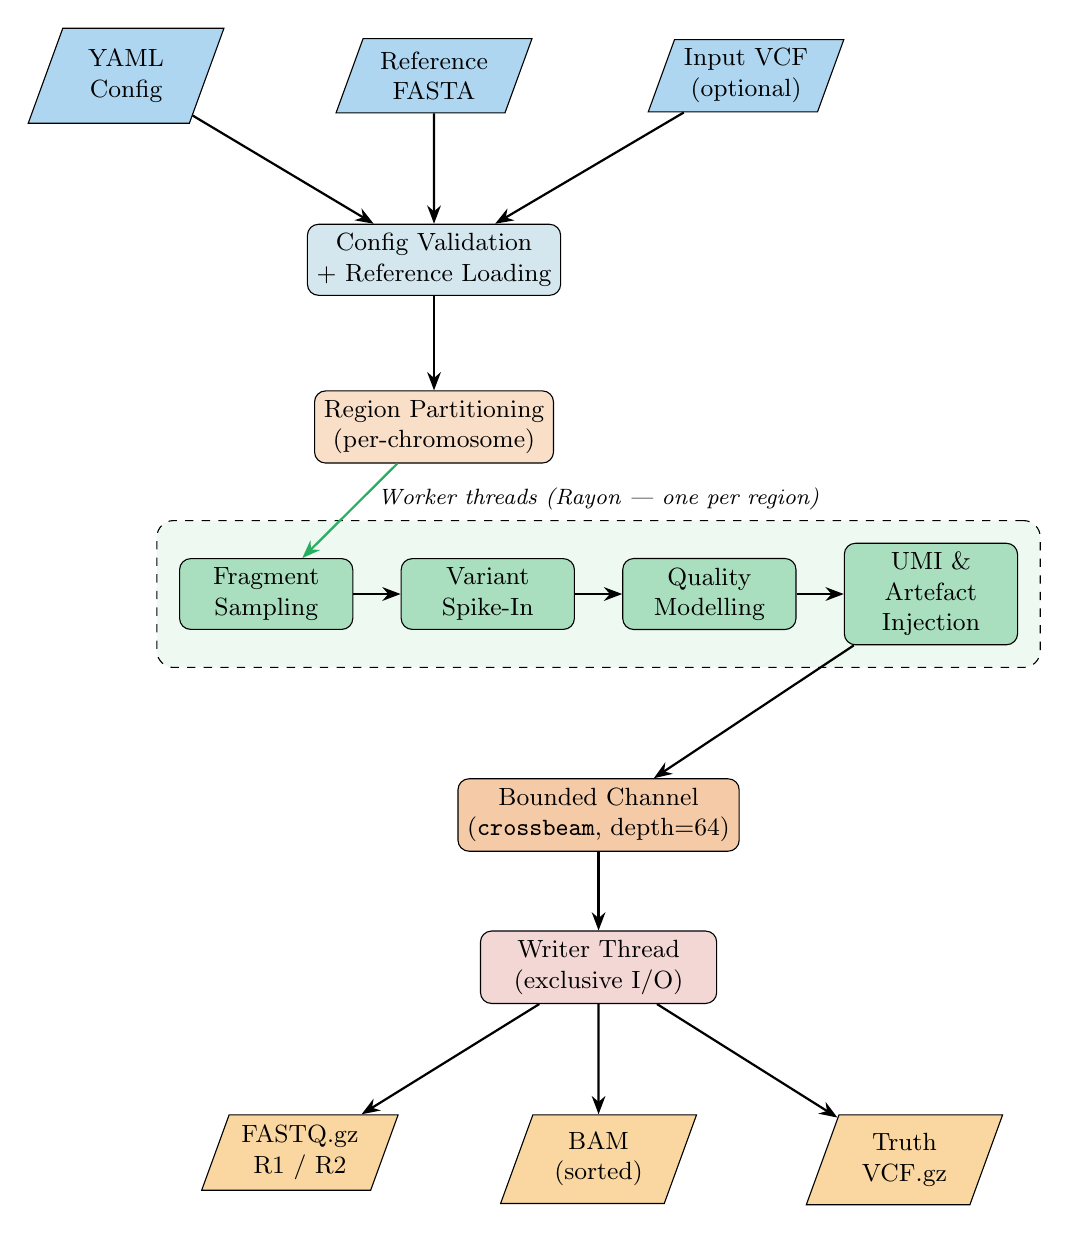
\begin{tikzpicture}[
    node distance = 1.6cm and 2.2cm,
    box/.style    = {draw, rounded corners=4pt, minimum width=3.0cm,
                     minimum height=0.8cm, align=center, font=\small},
    io/.style     = {draw, trapezium, trapezium left angle=70,
                     trapezium right angle=110, minimum width=2.5cm,
                     minimum height=0.7cm, align=center, font=\small},
    worker/.style = {draw, dashed, rounded corners=6pt, inner sep=8pt},
    arr/.style    = {-Stealth, thick},
    parr/.style   = {-Stealth, thick, color=pipegreen},
  ]

  %% Top-level inputs
  \node[io, fill=pipelightblue] (cfg)  {YAML\\Config};
  \node[io, fill=pipelightblue, right=1.8cm of cfg] (ref) {Reference\\FASTA};
  \node[io, fill=pipelightblue, right=1.8cm of ref] (vcf) {Input VCF\\(optional)};

  %% Config parsing / validation
  \node[box, fill=pipeblue!20, below=1.4cm of ref] (parse) {Config Validation\\+ Reference Loading};
  \draw[arr] (cfg) -- (parse);
  \draw[arr] (ref) -- (parse);
  \draw[arr] (vcf) -- (parse);

  %% Region partitioning
  \node[box, fill=pipeorange!25, below=1.2cm of parse] (part) {Region Partitioning\\(per-chromosome)};
  \draw[arr] (parse) -- (part);

  %% Worker box
  \node[box, fill=pipelightgreen, below left=1.2cm and -0.5cm of part,
        minimum width=2.2cm] (frag) {Fragment\\Sampling};
  \node[box, fill=pipelightgreen, right=0.6cm of frag,
        minimum width=2.2cm] (spike) {Variant\\Spike-In};
  \node[box, fill=pipelightgreen, right=0.6cm of spike,
        minimum width=2.2cm] (qual) {Quality\\Modelling};
  \node[box, fill=pipelightgreen, right=0.6cm of qual,
        minimum width=2.2cm] (art) {UMI \&\\Artefact\\Injection};

  %% Worker bounding box
  \begin{scope}[on background layer]
    \node[worker, fill=pipegreen!8,
          fit=(frag)(spike)(qual)(art),
          label={[font=\footnotesize\itshape]above:Worker threads (Rayon — one per region)}] (worker) {};
  \end{scope}

  %% Arrows from partitioner into worker
  \draw[parr] (part) -- (frag);

  %% Intra-worker flow
  \draw[arr] (frag)  -- (spike);
  \draw[arr] (spike) -- (qual);
  \draw[arr] (qual)  -- (art);

  %% Bounded channel
  \node[box, fill=pipeorange!40, below=1.4cm of worker,
        minimum width=3.5cm] (chan) {Bounded Channel\\(\texttt{crossbeam}, depth=64)};
  \draw[arr] (art) -- (chan);

  %% Writer thread
  \node[box, fill=pipered!20, below=1.0cm of chan,
        minimum width=3.0cm] (writer) {Writer Thread\\(exclusive I/O)};
  \draw[arr] (chan) -- (writer);

  %% Outputs
  \node[io, fill=pipeyellow!40, below left=1.4cm and 1.8cm of writer]  (fq)    {FASTQ.gz\\R1 / R2};
  \node[io, fill=pipeyellow!40, below=1.4cm of writer]                  (bam)   {BAM\\(sorted)};
  \node[io, fill=pipeyellow!40, below right=1.4cm and 1.8cm of writer] (truth) {Truth\\VCF.gz};

  \draw[arr] (writer) -- (fq);
  \draw[arr] (writer) -- (bam);
  \draw[arr] (writer) -- (truth);

\end{tikzpicture}
\caption{%
  \textbf{\varforge{} processing pipeline.}
  A validated YAML configuration drives reference loading, variant
  preparation, and genome partitioning.  Independent worker threads
  (managed by Rayon) process each region through fragment sampling,
  variant spike-in, quality score assignment, and UMI/artefact
  injection.  Completed region batches are sent through a bounded
  \texttt{crossbeam-channel} (default depth 64) to a dedicated writer
  thread, which owns all output handles exclusively and writes each
  batch to compressed FASTQ, coordinate-sorted BAM, and a truth VCF
  immediately upon receipt.
}
\label{fig:pipeline}
\end{figure}

\subsection{Configuration System}
\label{sec:methods:config}

\varforge{} is driven entirely by a YAML configuration file, allowing
all simulation parameters to be specified, version-controlled, and
shared without additional tooling.  Only two fields are mandatory
(\texttt{reference} and \texttt{output.directory}); all others carry
sensible defaults.  The composable feature blocks---\texttt{tumour},
\texttt{umi}, \texttt{artifacts}, \texttt{copy\_number},
\texttt{gc\_bias}, \texttt{capture}---are enabled by their presence in
the configuration and independently omissible; no feature carries
implicit overhead when not configured.

Named presets aggregate commonly used parameter combinations.
Domain-specific presets such as \texttt{cancer:melanoma} set biologically
motivated purity, mutation burden, and mutation-type fractions based on
published COSMIC mutational signatures.  Workflow presets such as
\texttt{cfdna} or \texttt{umi} configure fragment models and barcode
parameters for common benchmarking scenarios.  Preset values are
always overridden by explicit YAML fields.

A \texttt{validate} subcommand performs schema validation, cross-field
consistency checking (e.g., ensuring that variant type fractions sum to
exactly 1.0, that copy number regions do not exceed chromosome bounds),
and reference genome accessibility checks without executing any
simulation, enabling rapid configuration iteration.

\subsection{Read Generation Engine}
\label{sec:methods:reads}

\subsubsection{Fragment Sampling}
\label{sec:methods:reads:frags}

For standard whole-genome and panel sequencing, fragment lengths are
sampled from a normal distribution $\mathcal{N}(\mu, \sigma^2)$ with
user-configured mean $\mu$ and standard deviation $\sigma$.  A cfDNA
fragment model is detailed in Section~\ref{sec:methods:cfdna}.

For each sampled fragment, a genomic start position is drawn uniformly
at random from the active region.  Reads are oriented in the standard
paired-end convention: Read~1 maps to the forward strand at the
5$'$~end of the fragment; Read~2 maps to the reverse strand at the
3$'$~end.  Reads extending beyond chromosome boundaries are discarded.

\subsubsection{Quality Score Modelling}
\label{sec:methods:reads:qual}

\varforge{} implements two quality score models.

\textbf{Parametric model.}  Per-cycle quality scores are drawn from a
normal distribution with mean $\bar{Q}$ that decays linearly from
cycle to cycle:
\begin{equation}
  \bar{Q}(c) = Q_0 - \lambda \cdot c
  \label{eq:qual-decay}
\end{equation}
where $Q_0$ is the first-cycle mean quality, $\lambda$ is a per-cycle
decay constant, and $c$ is the zero-indexed cycle number.  Read~2 is
assigned a higher error rate than Read~1 by applying a fixed offset to
$Q_0$.  Given a drawn quality score $Q$, the sequencing error probability
is $p_e = 10^{-Q/10}$; an error is applied with probability $p_e$ by
substituting the base with a randomly chosen alternate drawn from the
three non-reference possibilities.

\textbf{Empirical model.}  When a user runs \texttt{varforge
learn-profile --bam <real.bam>}, \varforge{} parses the real BAM to
extract per-cycle, per-base-context quality score histograms and
substitution probability matrices.  The resulting JSON profile is
referenced from the \texttt{quality.profile\_path} configuration field
and replaces the parametric model at simulation time.  This mode
produces reads whose quality distributions are indistinguishable from
those of the training dataset at the level of base quality statistics.

\subsubsection{Stochastic VAF Sampling}
\label{sec:methods:reads:vaf}

A key methodological contribution of \varforge{} is the per-read
stochastic sampling of variant alleles.  For each read overlapping a
variant site, \varforge{} independently draws from a Bernoulli
distribution:
\begin{equation}
  X_i \sim \text{Bernoulli}(\text{VAF}_\text{eff})
  \label{eq:bernoulli}
\end{equation}
where $X_i = 1$ indicates that read $i$ carries the alt allele.  The
number of alt reads at depth $D$ therefore follows
\begin{equation}
  A \sim \text{Binomial}(D,\; \text{VAF}_\text{eff})
  \label{eq:binomial}
\end{equation}
rather than the deterministic $A = \lfloor D \cdot \text{VAF}_\text{eff}
\rfloor$ used by \bamsurgeon{} and SomatoSim.

This distinction is illustrated in Figure~\ref{fig:vaf-comparison}.
For a 10\% VAF variant at 30$\times$ coverage, the deterministic model
always produces exactly~3 alt reads.  \varforge{}'s stochastic model
produces a distribution centred on~3 with variance $D \cdot
\text{VAF}_\text{eff} \cdot (1 - \text{VAF}_\text{eff}) \approx 0.81$,
matching the natural sampling variability of a sequencing experiment.
At low depths or low VAFs the impact is more pronounced: the deterministic
model at 30$\times$ and 1\% VAF always produces 0 alt reads, while the
stochastic model correctly samples 0 or 1 alt reads with probability
$\sim$26\%.  Benchmarks built on deterministic data overestimate
sensitivity at low VAF precisely because the data never presents the
zero-coverage challenges that challenge real callers.

\begin{figure}[H]
\centering
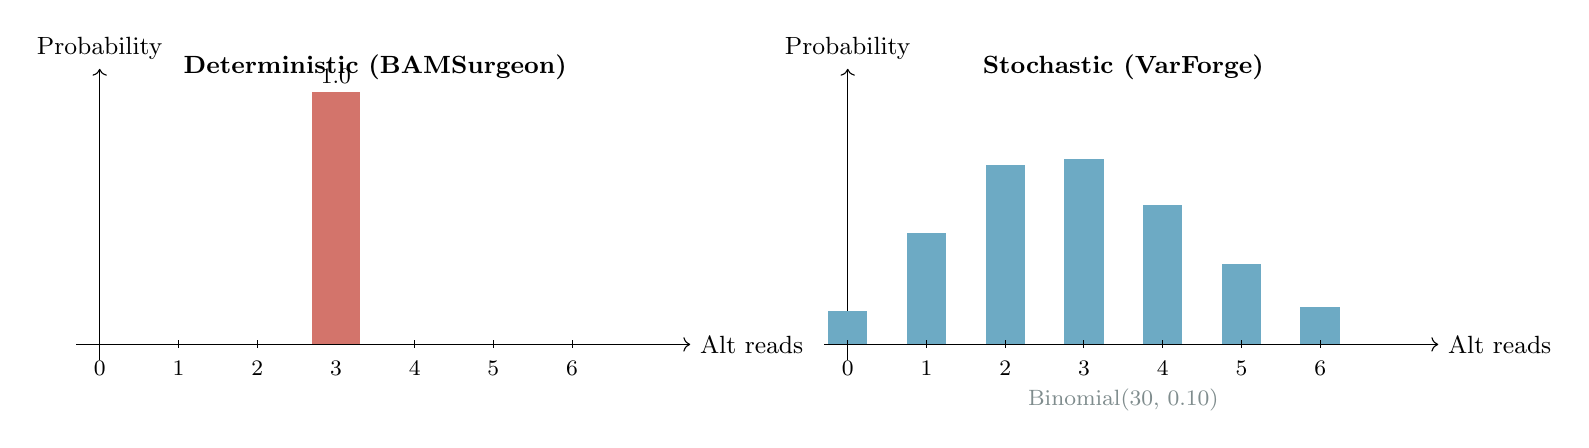
\begin{tikzpicture}[scale=1.0]
  %% --- Left panel: deterministic ---
  \begin{scope}
    \draw[->] (-0.3,0) -- (7.5,0) node[right, font=\small] {Alt reads};
    \draw[->] (0,-0.2) -- (0,3.5) node[above, font=\small] {Probability};
    \node[font=\small\bfseries, anchor=north] at (3.5,3.8)
      {Deterministic (BAMSurgeon)};
    %% single bar at x=3 (3 alt reads)
    \fill[pipered!70] (2.7,0) rectangle (3.3,3.2);
    \node[font=\footnotesize] at (3.0,-0.3) {3};
    \node[font=\footnotesize] at (3.0,3.4)  {1.0};
    %% x-axis ticks
    \foreach \x/\lbl in {0/0,1/1,2/2,4/4,5/5,6/6} {
      \draw (\x, 0.05) -- (\x,-0.05);
      \node[font=\footnotesize] at (\x,-0.3) {\lbl};
    }
  \end{scope}

  %% --- Right panel: stochastic ---
  \begin{scope}[xshift=9.5cm]
    \draw[->] (-0.3,0) -- (7.5,0) node[right, font=\small] {Alt reads};
    \draw[->] (0,-0.2) -- (0,3.5) node[above, font=\small] {Probability};
    \node[font=\small\bfseries, anchor=north] at (3.5,3.8)
      {Stochastic (VarForge)};
    %% Approximate Binomial(30, 0.10) bars
    %% P(k) values (approx): k=0:0.042, 1:0.141, 2:0.228, 3:0.236, 4:0.177, 5:0.102, 6:0.047
    \foreach \x/\h in {0/0.42, 1/1.41, 2/2.28, 3/2.36, 4/1.77, 5/1.02, 6/0.47} {
      \fill[pipeblue!70] (\x-0.3+0.05,0) rectangle (\x+0.3-0.05,\h);
    }
    \foreach \x in {0,1,2,3,4,5,6} {
      \draw (\x, 0.05) -- (\x,-0.05);
      \node[font=\footnotesize] at (\x,-0.3) {\x};
    }
    \node[font=\footnotesize, color=pipegray] at (3.5, -0.7)
      {Binomial$(30,\, 0.10)$};
  \end{scope}
\end{tikzpicture}
\caption{%
  \textbf{Deterministic versus stochastic VAF spike-in at 10\% VAF,
  30$\times$ coverage.}
  Left: \bamsurgeon{}-style deterministic spike-in always places exactly
  3 alt reads, presenting an unrealistically clean signal to variant
  callers.
  Right: \varforge{}'s per-read Bernoulli sampling produces alt-read
  counts drawn from Binomial$(30, 0.10)$, faithfully reproducing the
  natural sampling variance of real sequencing.
}
\label{fig:vaf-comparison}
\end{figure}

\subsection{Variant Spike-In}
\label{sec:methods:variants}

\subsubsection{Small Variants: SNVs, Indels, and MNVs}
\label{sec:methods:variants:small}

For SNVs, the reference base in each selected read is replaced with the
alternate allele.  The quality score assigned to the substituted position
is drawn from the distribution of the surrounding positions rather than
set to a fixed value, preserving the local quality context.

Indels are applied by modifying both the read sequence and the CIGAR
string.  Insertions are handled by splicing new bases into the read
sequence and appending an \texttt{I} operation to the CIGAR.  Deletions
remove bases from the read and insert a \texttt{D} operation.  Following
indel application, \varforge{} performs local re-alignment using
Smith-Waterman to produce a correct, minimal CIGAR string that resolves
the left-alignment convention and avoids read soft-clipping where
unnecessary.

MNVs present a specific phasing challenge: two or more adjacent SNVs must
appear on the \emph{same} read rather than being independently distributed
across reads.  \varforge{} groups MNV components into a single compound
event and applies all substitutions atomically to each selected read,
ensuring correct cis-phase representation.

\subsubsection{Structural Variants}
\label{sec:methods:variants:sv}

\varforge{} supports five canonical SV classes: deletion, insertion,
inversion, tandem duplication, and inter-chromosomal translocation.  Each
class is realised by generating both split reads and discordant
read pairs at the breakpoints.  Split reads are rendered as soft-clipped
primary alignments with supplementary alignment records (\texttt{SA}
tags) pointing to the breakpoint partner.  Discordant pairs have
unexpected insert sizes (deletions), unexpected orientation (inversions),
or mates on different chromosomes (translocations).  CIGAR strings,
mate coordinates, and auxiliary tags are set to values consistent with
BWA-MEM~\citep{li2009bwa} output conventions so that reads are
correctly processed by downstream SV callers.

\subsubsection{Copy Number Variants}
\label{sec:methods:variants:cnv}

Copy number alterations are modelled as regions of the genome where the
read depth deviates from the genome-wide target in proportion to the
local tumour copy number.  For a region with tumour copy number
$\text{CN}_\text{tumor}$ and normal copy number $\text{CN}_\text{normal} = 2$,
at sample purity $p$, the expected depth multiplier relative to the
diploid baseline is:
\begin{equation}
  \text{depth\_multiplier} =
    \frac{p \cdot \text{CN}_\text{tumor} + (1-p) \cdot 2}{2}
  \label{eq:cn-depth}
\end{equation}
Fragment start positions within CNV regions are sampled at a rate
scaled by this multiplier.  \varforge{} also adjusts the effective VAF
of any somatic variant overlapping a CNV region according to the full
VAF equation (Section~\ref{sec:methods:tumour:vaf}).

\subsection{Tumour Modelling}
\label{sec:methods:tumour}

\subsubsection{Clonal Tree Architecture}
\label{sec:methods:tumour:clones}

Tumour heterogeneity is represented as a directed tree of clones.  Each
node in the tree carries a cancer cell fraction (CCF) and a set of
somatic mutations.  Mutations accumulate down the tree: a variant
assigned to an internal node is present in all descendant clones as
well.  The configuration accepts an arbitrary-depth tree, enabling
models ranging from a single clonal population to complex multi-branch
subclonal architectures.  \varforge{} validates that the CCF of child
nodes does not exceed the CCF of their parent and that the sum of CCFs
in any set of sibling branches does not exceed the parent CCF, ensuring
a biologically admissible clonal composition.

\subsubsection{Purity and Ploidy Integration}
\label{sec:methods:tumour:vaf}

The expected variant allele frequency for a somatic mutation is
computed from the cancer genomics VAF equation:
\begin{equation}
  \text{VAF}_\text{eff} =
    \frac{\text{CCF} \times m \times p}
         {p \cdot \text{CN}_\text{tumor} + (1-p) \cdot \text{CN}_\text{normal}}
  \label{eq:vaf}
\end{equation}
where $m$ is the multiplicity (number of mutant allele copies per
carrier cell), $p$ is the tumour purity, and $\text{CN}_\text{normal}$
is typically~2.  In the common case of a clonal heterozygous SNV in a
diploid tumour at 60\% purity, Equation~\ref{eq:vaf} gives
$\text{VAF}_\text{eff} = 0.30$.  The equation correctly handles
sub-clonal variants ($\text{CCF} < 1$), copy number gains
($\text{CN}_\text{tumor} > 2$), and loss of heterozygosity
($\text{CN}_\text{tumor} = 1$, $m = 1$), as well as extreme low tumour
fractions representative of liquid biopsy ($p \ll 0.1$).

A matched normal sample can be generated by setting purity to zero,
producing a diploid genome without somatic variants, using the same
reference sequence and random seed as the tumour to ensure consistent
germline background.

\subsection{UMI and Duplex Sequencing Simulation}
\label{sec:methods:umi}

\subsubsection{Barcode Generation and Error Injection}
\label{sec:methods:umi:barcodes}

Each original template molecule is assigned a unique molecular identifier
(UMI) of configurable length (typically 8--12 nucleotides).  The UMI
sequence is drawn by sampling each base independently and uniformly from
$\{A, C, G, T\}$.  A UMI sequencing error is then applied independently
to each base of the UMI with probability $p_\text{UMI}$ (default: 1\%
per base), producing the slightly corrupted UMI sequence that is observed
in the read.  The \texttt{RX} BAM tag stores the observed UMI sequence;
the \texttt{MI} tag records the true molecule identifier.  UMIs can be
delivered inline (prepended to the read sequence) or in the read name,
matching the conventions of fgbio and UMI-tools respectively.

\subsubsection{PCR Family Size Modelling}
\label{sec:methods:umi:families}

Each original molecule is amplified through a configurable number of
PCR cycles.  The family size (number of reads originating from a single
molecule) follows a log-normal distribution:
\begin{equation}
  F \sim \text{LogNormal}(\mu_F,\, \sigma_F^2)
  \label{eq:family-size}
\end{equation}
with parameters calibrated to reproduce the skewed, right-tailed family
size distributions observed in real UMI libraries.  All reads within a
family share the same molecule start and end coordinates and the same
(possibly error-containing) UMI sequence; each read independently
acquires sequencing errors during quality score assignment, consistent
with independent sequencing of PCR copies.

\subsubsection{Simplex and Duplex Strand Pairing}
\label{sec:methods:umi:duplex}

In duplex mode~\citep{schmitt2012duplex}, each original double-stranded
molecule yields two complementary strand families.  The top strand is
assigned UMI pair $(\alpha, \beta)$; the bottom strand is assigned the
swapped pair $(\beta, \alpha)$.  Downstream consensus-calling tools
(fgbio \texttt{CallDuplexConsensusReads}, duplex-seq-pipeline) use
this swapping convention to identify paired SSCS families and build
duplex consensus reads.  \varforge{} correctly propagates somatic
variants to \emph{both} strands so that true mutations survive
duplex consensus, while simulated sequencing artefacts (FFPE, oxoG)
are applied strand-specifically so that they are correctly eliminated
by the duplex consensus algorithm, faithfully reproducing the error
suppression logic that makes duplex sequencing valuable.

\subsection{Cell-Free DNA Fragmentation}
\label{sec:methods:cfdna}

\subsubsection{Nucleosomal Mixture Model}
\label{sec:methods:cfdna:mixture}

When the \texttt{cfda} fragment model is selected, \varforge{} samples
fragment lengths from a mixture of Gaussian components reflecting
nucleosomal protection:
\begin{equation}
  P(L) = \sum_{k=1}^{K} w_k \cdot \mathcal{N}(L;\, \mu_k,\, \sigma_k^2)
  \label{eq:cfdna-mixture}
\end{equation}
with four components representing the sub-nucleosomal shoulder
($\mu_1 \approx 143\,\text{bp}$, $w_1 \approx 0.08$), the dominant
mono-nucleosomal peak ($\mu_2 \approx 167\,\text{bp}$, $w_2 \approx 0.85$),
the di-nucleosomal component ($\mu_3 \approx 334\,\text{bp}$, $w_3
\approx 0.05$), and the tri-nucleosomal component ($\mu_4 \approx
500\,\text{bp}$, $w_4 \approx 0.02$).

\subsubsection{10\,bp Periodicity}
\label{sec:methods:cfdna:periodicity}

The 10\,bp helical-pitch periodicity of DNA wound around the histone
octamer manifests as regular oscillations in cfDNA fragment length
distributions below 167\,bp~\citep{snyder2016cfdna_nucleosome}.
\varforge{} models this by multiplying the mixture density by a
sinusoidal modulation:
\begin{equation}
  P'(L) \propto P(L) \cdot \bigl[1 + A\,\sin\!\bigl(2\pi L / 10.4\bigr)\bigr]
  \label{eq:periodicity}
\end{equation}
where the amplitude $A$ (default: 0.15) and period (10.4\,bp,
matching the known helical repeat) are configurable.  The modulated
density is re-normalised before sampling.

\subsubsection{ctDNA Enrichment}
\label{sec:methods:cfdna:ctdna}

Tumour-derived cfDNA fragments are shorter than non-tumour cfDNA,
with a characteristic peak near 143--147\,bp and reduced representation
above 167\,bp~\citep{lo2010cfdna}.  \varforge{} models this by assigning
different mixture parameters to tumour-derived and normal-cell-derived
fragments.  For tumour-derived fragments (i.e., reads originating from
the tumour genome under the configured purity), the sub-nucleosomal
weight $w_1$ is increased and the mono-nucleosomal mean $\mu_2$ is
shifted downward by a configurable offset (default: 20\,bp).  This
produces the fragment-length bimodality between tumour and normal
contributions that cfDNA analysis tools such as
DELFI~\citep{cristiano2019delfi} exploit.

\begin{figure}[H]
\centering
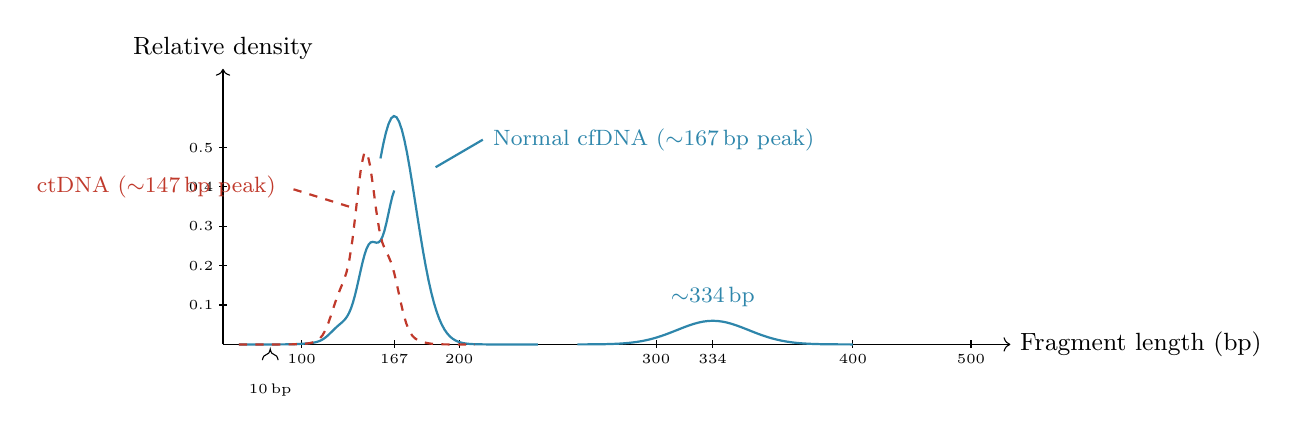
\begin{tikzpicture}[scale=1.0, yscale=5.0]
  %% Draw approximate cfDNA mixture density
  %% x-axis: fragment length 80-550bp
  \draw[->] (0,0) -- (10.0,0) node[right, font=\small] {Fragment length (bp)};
  \draw[->] (0,0) -- (0,0.70) node[above, font=\small] {Relative density};

  %% x-axis ticks
  \foreach \xlbl/\xpos in {100/1.0, 167/2.175, 200/3.0, 300/5.5, 334/6.22, 400/8.0, 500/9.5} {
    \draw (\xpos, 0.01) -- (\xpos, -0.01);
    \node[font=\tiny, below] at (\xpos,0) {\xlbl};
  }

  %% y-axis ticks
  \foreach \y in {0.1,0.2,0.3,0.4,0.5} {
    \draw (0.05,\y) -- (-0.05,\y);
    \node[font=\tiny, left] at (0,\y) {\y};
  }

  %% 10bp periodicity oscillations (simplified) below 167bp
  %% Draw as a wavy line in region 80-167bp
  \draw[thick, pipeblue, domain=0.2:2.175, samples=80]
    plot (\x, {0.35 * exp(-(\x-2.175)^2 / 0.25) * (1 + 0.15*sin((\x * 10.4 / 0.7) r))});

  %% Main mono-nucleosomal peak at 167bp (x=2.175 on our scale where 10bp = 0.13 units)
  %% Let scale: 100bp -> 1.0, 550bp -> 10, so 1bp = 0.0182 units
  %% 167bp -> 2.175, sigma~15bp -> 0.273 units
  \draw[thick, pipeblue, domain=2.0:4.0, samples=60]
    plot (\x, {0.58 * exp(-(\x-2.175)^2 / (2*0.273^2))});

  %% Di-nucleosomal at 334bp -> 6.22, sigma~25bp -> 0.455 units, weight 0.05
  \draw[thick, pipeblue, domain=4.5:8.0, samples=60]
    plot (\x, {0.06 * exp(-(\x-6.22)^2 / (2*0.455^2))});

  %% ctDNA shifted component
  \draw[thick, pipered, dashed, domain=0.2:3.2, samples=80]
    plot (\x, {0.42 * exp(-(\x-1.84)^2 / (2*0.24^2)) *
               (1 + 0.18*sin((\x * 10.4 / 0.7) r))});

  %% Labels
  \draw[pipeblue, thick] (2.7,0.45) -- (3.3,0.52)
    node[right, font=\footnotesize, color=pipeblue]
    {Normal cfDNA ($\sim$167\,bp peak)};
  \draw[pipered, thick, dashed] (1.6,0.35) -- (0.8,0.40)
    node[left, font=\footnotesize, color=pipered]
    {ctDNA ($\sim$147\,bp peak)};

  %% 10bp brace
  \draw[decorate, decoration={brace, amplitude=4pt}]
    (0.5,-0.04) -- (0.7,-0.04)
    node[midway, below=5pt, font=\tiny] {10\,bp};

  %% Di-nucleosomal label
  \node[font=\footnotesize, color=pipeblue] at (6.22, 0.12)
    {$\sim$334\,bp};

\end{tikzpicture}
\caption{%
  \textbf{\varforge{} cfDNA fragment length model.}
  The normal cfDNA mixture (solid blue) comprises a dominant
  mono-nucleosomal peak at $\sim$167\,bp, a di-nucleosomal component
  at $\sim$334\,bp, and sub-nucleosomal oscillations below 167\,bp
  with 10\,bp periodicity matching the DNA helical repeat.
  Tumour-derived ctDNA fragments (dashed red) are shifted toward
  shorter lengths with a peak near $\sim$143--147\,bp, enabling
  fragment-length-based tumour fraction estimation by tools such as
  DELFI and ichorCNA.
}
\label{fig:cfdna}
\end{figure}

\subsection{Library Artefact Simulation}
\label{sec:methods:artefacts}

\subsubsection{FFPE Deamination}
\label{sec:methods:artefacts:ffpe}

FFPE-induced cytosine deamination is modelled by applying C$>$T
(and complementary G$>$A) substitutions to read bases at a
configurable rate $r_\text{FFPE}$ (default when enabled: 2\%).
Deamination occurs preferentially on single-stranded overhang regions
at fragment ends; \varforge{} applies a higher substitution rate to the
first and last 5 bases of each read and a lower rate to internal bases,
consistent with the biochemical mechanism and the strand-bias signatures
observed in FFPE tumour sequencing.  The artefacts are applied
\emph{after} variant spike-in, so that FFPE-induced C$>$T transitions are
distinguishable from true somatic SNVs via the \texttt{tp} BAM tag.

\subsubsection{Oxidative Damage}
\label{sec:methods:artefacts:oxog}

8-oxoguanine (8-oxoG) damage produces G$>$T transversions (C$>$A on
the complementary strand) with a characteristic OxoG-type strand bias.
\varforge{} models this by applying G$>$T substitutions on Read~1 and
C$>$A substitutions on Read~2 at a configurable rate $r_\text{OxoG}$,
consistent with the oxidation pattern arising during library preparation
that fgbio's \texttt{FilterConsensusReads} is designed to eliminate.

\subsubsection{PCR Duplicates and Errors}
\label{sec:methods:artefacts:pcr}

PCR amplification introduces two types of noise.  Duplicate molecules
arise when a template is amplified more than once and both copies are
sequenced; \varforge{} generates duplicate read families from a
log-normal amplification distribution (Section~\ref{sec:methods:umi:families})
rather than injecting copies at a fixed duplicate rate.  This produces
a more realistic family-size distribution that reflects true PCR
kinetics.  PCR substitution errors are applied independently to each
PCR copy at a configurable per-cycle error rate (default: $10^{-3}$
per base per cycle), producing errors that appear on all downstream
copies of an affected template---the signature that distinguishes early-
from late-cycle PCR errors.

\subsubsection{GC Bias}
\label{sec:methods:artefacts:gcbias}

GC bias is modelled as a fragment-level coverage multiplier that reduces
the sampling probability for fragments with extreme GC content.  The
default model applies an empirical U-shaped weighting function with
suppression below 30\% GC and above 70\% GC, matching the bias profiles
observed in real Illumina library preparations and learned by
ReSeq~\citep{schmeing2021reseq}.  Users may specify a \texttt{severity}
multiplier to amplify or suppress the bias, or apply a flat model for
unbiased simulation.

\subsection{BAM Editing Mode}
\label{sec:methods:edit}

In addition to de-novo simulation, \varforge{} provides a
\texttt{varforge edit} subcommand that spikes variants from a VCF
directly into an existing BAM file, analogous to \bamsurgeon{}.  This
mode is appropriate when the user wishes to add a small number of known
mutations to a real-data or previously simulated BAM while preserving
the authentic read background.

Compared to \bamsurgeon{}, \varforge{}'s editing mode differs in three
important respects.  First, it applies stochastic VAF sampling
(Section~\ref{sec:methods:reads:vaf}) rather than deterministic
modification.  Second, it is UMI-family-aware: when the input BAM
contains UMI tags, \varforge{} selects reads for modification at the
molecule (family) level, ensuring that all reads in a molecule either
carry or do not carry the variant, consistent with the biological fact
that a mutation is present in the original template rather than
appearing independently in PCR copies.  Third, it avoids the local
assembly step used by \bamsurgeon{} for SVs, instead directly
constructing split-read and discordant-pair records, which is both
faster and avoids the imprecise breakpoint placement that is a known
limitation of \bamsurgeon{}'s local assembly.

\subsection{Implementation}
\label{sec:methods:impl}

\subsubsection{Rust for Performance and Safety}
\label{sec:methods:impl:rust}

\varforge{} is implemented entirely in Rust, a systems programming
language that achieves performance comparable to C and C++ while
providing memory safety guarantees through its ownership type system.
The single-binary distribution requires no runtime installation
(no JVM, no Python interpreter, no dynamic shared libraries) and
is available as pre-built binaries for Linux (x86\_64, aarch64) and
macOS (Apple Silicon).

\subsubsection{Parallel Region Processing}
\label{sec:methods:impl:parallel}

The genome is partitioned into independent regions (by default, one per
chromosome).  Workers are spawned via the Rayon~\citep{rayon}
work-stealing scheduler, which dynamically balances load across
available cores without requiring manual thread management.  Each
worker has an independent random number generator seeded from a hash of
the global seed and the region identifier:
\begin{equation}
  \text{seed}_r = H(\text{seed}_\text{global},\, r)
  \label{eq:seed}
\end{equation}
This scheme ensures that (i) simulations are fully reproducible given
the same global seed and thread count, and (ii) adding or removing
regions does not perturb the output of unaffected regions---a
desirable property for differential benchmarking experiments.

\subsubsection{Streaming I/O Architecture}
\label{sec:methods:impl:io}

\varforge{} never holds the complete simulated dataset in memory.
Each worker thread assembles a \texttt{RegionBatch}---a \texttt{Vec}
of read pairs together with the variants applied in that region---and
sends it through a bounded \texttt{crossbeam-channel} to a dedicated
writer thread.  The channel depth is configurable via the
\texttt{performance.output\_buffer\_regions} parameter (default: 64
slots).  The writer thread owns the FASTQ and BAM output handles
exclusively, writing each batch immediately upon receipt and releasing
the batch memory.  This design bounds peak memory to
$\text{buffer\_depth} \times \text{batch\_size}$ regardless of the
total dataset size.  FASTQ output is compressed with
\texttt{flate2} (using the pure-Rust \texttt{rust\_backend}).  BAM
output is written through \texttt{noodles}~\citep{noodles}, a
pure-Rust implementation of the SAM/BAM/CRAM specification that avoids
the C library FFI overhead of the alternative \texttt{rust-htslib}
binding.

\subsubsection{Pure Rust Dependency Stack}
\label{sec:methods:impl:deps}

All I/O is handled by pure-Rust crates: \texttt{noodles}~\citep{noodles}
for BAM, SAM, VCF, FASTA, and BED; \texttt{seq\_io}~\citep{seqio} for
zero-allocation FASTQ writing; and \texttt{serde\_yaml}~\citep{serde}
for configuration parsing.  Statistical sampling uses
\texttt{rand\_distr} for all distributions (normal, log-normal,
binomial, Bernoulli), with \texttt{statrs} for any distribution
evaluations required during parameter fitting.  The CLI is implemented
with \texttt{clap}~\citep{clap} and structured logging with
\texttt{tracing}, which supports JSON output for machine-readable
pipeline logging.  The absence of C-library dependencies eliminates
build-environment variability and simplifies cross-compilation.

%%────────────────────────────────────────────────────────────────────────────
%%  4. Results
%%────────────────────────────────────────────────────────────────────────────
\section{Results}
\label{sec:results}

\subsection{Experimental Setup}
\label{sec:results:setup}

All benchmarks were executed on a single workstation equipped with an AMD
Ryzen 5 7640HS (6 cores / 12 threads, 5.0\,GHz boost), 12\,GiB DDR5 RAM,
and a 454\,GB NVMe SSD running Debian GNU/Linux~13 (kernel 6.12.74).
\varforge{} v0.1.0 was compiled with \texttt{rustc}~1.94.0 in release
mode without profile-guided optimisation.

Synthetic reference FASTA files were generated by a reproducible Python
script rather than using a licensed genome, controlling for reference GC
content ($\approx$40\%) and eliminating download dependencies.  Three
reference sizes were used: 1\,MB (6 chromosomes), 10\,MB (8 chromosomes),
and 50\,MB (12 chromosomes).  Twelve named configurations (Table~\ref{tab:scenarios})
covered the breadth of \varforge{}'s feature set.  Configurations
generating fewer than $\sim$2M read pairs received three iterations;
larger configurations received one iteration due to time and memory
constraints on the 12\,GiB test system.  All reported times are mean
wall-clock times captured with \texttt{busybox time -v}.  Benchmarks
collected on 2026-03-16.

\subsection{Throughput Benchmarks}
\label{sec:results:throughput}

Table~\ref{tab:scenarios} summarises all twelve scenario benchmarks.  At
the baseline configuration (10\,MB reference, 30$\times$, no optional
features, 12 threads), \varforge{} produces approximately 1.26M read pairs
in 75.4 seconds, corresponding to a wall-clock throughput of
$\sim$13{,}400 read pairs per second, or $\sim$4.0\,Gbp/min of raw
sequence.  Variant spike-in of 500 mutations adds less than one second
(+0.6\%), confirming that variant lookup and Bernoulli application
contribute negligible overhead at this scale.

The higher per-read throughput observed on the 1\,MB reference
($\sim$28{,}000 read pairs/sec at $\geq$30$\times$; see
Section~\ref{sec:results:coverage}) reflects a compute-bound regime where
the write pipeline is no longer the bottleneck.  The 10\,MB and 50\,MB
baselines converge to the same $\sim$13{,}400 read pairs/sec,
indicating that FASTQ compression and NVMe write latency dominate at
those reference sizes and coverage depths.

The cfDNA run (1\,MB, 200$\times$, 2\% purity) achieves $\sim$14{,}100
read pairs/sec.  The FFPE run (10\,MB, 30$\times$) is counter-intuitively
slightly faster on a per-read basis ($\sim$14{,}400 read pairs/sec)
because the per-base damage pass produces shorter effective inserts,
increasing reads per fragment.

\begin{table}[H]
\centering
\caption{%
  \textbf{Main scenario benchmarks.}
  All runs use 12 threads.  Peak RAM marked with $\dagger$ exceeded
  12\,GiB physical memory; swap was used and times are degraded.
  ``Read pairs/sec'' is the wall-clock throughput.
}
\label{tab:scenarios}
\small
\begin{tabular}{llrrlrr r}
\toprule
Config & Ref & Cov & Variants & Features & Iters
       & Avg Wall (s) & Peak RAM (MB) \\
\midrule
01\_baseline           & 10\,MB & 30$\times$  & none  & none                     & 3 & 75.4  & 3{,}421 \\
02\_with\_variants     & 10\,MB & 30$\times$  & 500   & none                     & 3 & 75.9  & 3{,}423 \\
03\_high\_coverage     & 10\,MB & 100$\times$ & 500   & none                     & 1 & 251.1 & 11{,}352 \\
04\_very\_high\_cov    & 1\,MB  & 200$\times$ & 100   & none                     & 3 & 47.8  & 2{,}271 \\
05\_umi\_simplex       & 10\,MB & 100$\times$ & none  & UMI simplex              & 1 & 376.1 & 35{,}552$^\dagger$ \\
06\_umi\_duplex        & 10\,MB & 100$\times$ & none  & UMI duplex               & 1 & 373.6 & 35{,}553$^\dagger$ \\
07\_cfdna             & 1\,MB  & 200$\times$ & 200   & cfDNA, 2\% purity         & 3 & 47.5  & 2{,}382 \\
08\_ffpe\_artifacts    & 10\,MB & 30$\times$  & 500   & FFPE + oxoG              & 3 & 87.5  & 4{,}547 \\
09\_all\_features      & 10\,MB & 100$\times$ & 500   & all                      & 1 & 471.0 & 39{,}521$^\dagger$ \\
10\_large\_genome      & 50\,MB & 30$\times$  & 1{,}000 & none                   & 1 & 374.5 & 16{,}846$^\dagger$ \\
11\_panel\_simulation  & 1\,MB  & 200$\times$ & 50    & UMI simplex              & 3 & 76.8  & 7{,}161 \\
12\_ultra\_deep        & 1\,MB  & 500$\times$ & 20    & UMI duplex               & 1 & 190.5 & 17{,}901$^\dagger$ \\
\bottomrule
\end{tabular}
\end{table}

\subsection{Thread Scaling}
\label{sec:results:scaling}

Thread scaling was evaluated on the \texttt{02\_with\_variants} configuration
(10\,MB reference, 30$\times$, 500 variants) from 1 to 12 threads.
Table~\ref{tab:threads} presents the results; Figure~\ref{fig:thread-scaling}
plots the speedup curve.

\begin{table}[H]
\centering
\caption{%
  \textbf{Thread scaling.}
  Configuration: 10\,MB reference, 30$\times$ coverage, 500 variants.
  Speedup is relative to the single-thread run (86.0\,s).
}
\label{tab:threads}
\small
\begin{tabular}{rrr r}
\toprule
Threads & Avg Wall (s) & Speedup & Efficiency \\
\midrule
1  & 86.0 & 1.00$\times$ & 100\% \\
2  & 75.8 & 1.13$\times$ &  57\% \\
4  & 74.0 & 1.16$\times$ &  29\% \\
6  & 74.3 & 1.16$\times$ &  19\% \\
8  & 75.1 & 1.14$\times$ &  14\% \\
12 & 75.7 & 1.14$\times$ &  10\% \\
\bottomrule
\end{tabular}
\end{table}

\begin{figure}[H]
\centering
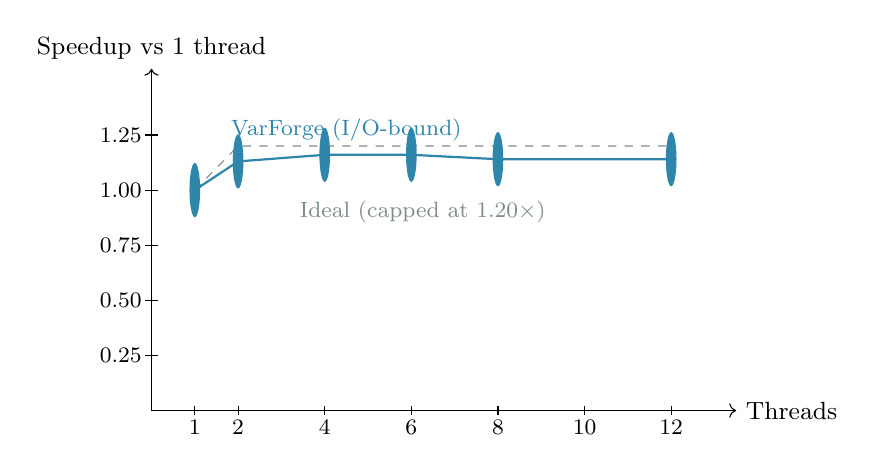
\begin{tikzpicture}
  \begin{scope}[xscale=0.55, yscale=2.8]
    %% Axes
    \draw[->] (0,0) -- (13.5,0) node[right, font=\small] {Threads};
    \draw[->] (0,0) -- (0,1.55) node[above, font=\small] {Speedup vs 1 thread};

    %% Ideal dashed line (capped at 1.20 for legibility)
    \draw[dashed, pipegray, domain=1:12, samples=12]
      plot (\x, {min(\x, 1.20)});
    \node[font=\footnotesize, color=pipegray, anchor=west] at (3.2, 0.90)
      {Ideal (capped at 1.20$\times$)};

    %% Actual speedup data: (threads, speedup)
    \foreach \t/\s in {1/1.00, 2/1.13, 4/1.16, 6/1.16, 8/1.14, 12/1.14} {
      \fill[pipeblue] (\t, \s) circle (3.5pt);
    }
    \draw[pipeblue, thick]
      (1,1.00) -- (2,1.13) -- (4,1.16) -- (6,1.16) -- (8,1.14) -- (12,1.14);

    %% x-axis ticks
    \foreach \t in {1,2,4,6,8,10,12} {
      \draw (\t, 0.02) -- (\t, -0.02);
      \node[font=\footnotesize, below] at (\t, 0) {\t};
    }
    %% y-axis ticks
    \foreach \s in {0.25,0.50,0.75,1.00,1.25} {
      \draw (0.15,\s) -- (-0.15,\s);
      \node[font=\footnotesize, left] at (0, \s) {\s};
    }

    \node[pipeblue, font=\footnotesize, anchor=south] at (4.5, 1.18)
      {VarForge (I/O-bound)};
  \end{scope}
\end{tikzpicture}
\caption{%
  \textbf{Thread scaling on the 10\,MB / 30$\times$ / 500-variant
  configuration.}
  The speedup plateau at $\approx$1.16$\times$ above 2 threads
  indicates that the workload at this scale is I/O-bound: FASTQ
  compression and NVMe writes saturate the storage pipeline before
  additional cores provide further benefit.  The dashed line shows the
  theoretical ideal (capped at 1.20$\times$ for legibility).
}
\label{fig:thread-scaling}
\end{figure}

Thread scaling for the 10\,MB / 30$\times$ configuration plateaus sharply
beyond 2 threads: the single-thread run is $\sim$14\% slower than
the multi-thread runs, but moving from 2 to 12 threads provides no
additional benefit.  The likely explanation is that writing
$\sim$280\,MB of compressed FASTQ (R1$+$R2) saturates the NVMe write
pipeline regardless of how many cores are generating sequences.  For
workloads with a higher compute-to-I/O ratio---larger references,
higher coverage, or UMI/artefact features---thread scaling is expected
to improve.  The all-features run (09) at 10\,MB $\times$ 100$\times$
generates roughly 10$\times$ more data per unit time, placing it in a
more compute-intensive regime where parallelism would yield greater
benefit.

\subsection{Coverage Scaling}
\label{sec:results:coverage}

Coverage scaling was measured on a 1\,MB reference with 100 random
mutations across depths from 1$\times$ to 200$\times$.
Table~\ref{tab:coverage} and Figure~\ref{fig:coverage-scaling} summarise
the results.

\begin{table}[H]
\centering
\caption{%
  \textbf{Coverage scaling on a 1\,MB reference with 100 random mutations.}
  Three iterations each.  Read pairs shown are approximate.
}
\label{tab:coverage}
\small
\begin{tabular}{rrr r r}
\toprule
Coverage & Approx.\ read pairs & Avg Wall (s) & Avg Peak RAM (MB) & Read pairs/sec \\
\midrule
  1$\times$ &     6{,}735 &  0.3 &     37 & $\sim$22{,}450 \\
  5$\times$ &    33{,}675 &  1.3 &     81 & $\sim$25{,}900 \\
 10$\times$ &    67{,}350 &  2.5 &    137 & $\sim$26{,}940 \\
 30$\times$ &   202{,}050 &  7.2 &    362 & $\sim$28{,}063 \\
 50$\times$ &   336{,}750 & 11.9 &    586 & $\sim$28{,}382 \\
100$\times$ &   673{,}335 & 23.8 &  1{,}146 & $\sim$28{,}291 \\
200$\times$ & 1{,}346{,}670 & 47.7 &  2{,}271 & $\sim$28{,}231 \\
\bottomrule
\end{tabular}
\end{table}

\begin{figure}[H]
\centering
\begin{tikzpicture}
  %% Wall-time panel
  \begin{scope}[xscale=0.055, yscale=0.10]
    \draw[->] (0,0) -- (215,0) node[right, font=\small] {Coverage ($\times$)};
    \draw[->] (0,0) -- (0,55)  node[above, font=\small] {Wall time (s)};

    %% Data points: (coverage, wall_time)
    \foreach \c/\t in {1/0.3, 5/1.3, 10/2.5, 30/7.2, 50/11.9, 100/23.8, 200/47.7} {
      \fill[pipeblue] (\c, \t) circle (5pt);
    }
    \draw[pipeblue, thick]
      (1,0.3) -- (5,1.3) -- (10,2.5) -- (30,7.2) -- (50,11.9) -- (100,23.8) -- (200,47.7);

    %% x ticks
    \foreach \c in {0,50,100,150,200} {
      \draw (\c, 0.5) -- (\c, -0.5);
      \node[font=\footnotesize, below] at (\c, 0) {\c};
    }
    %% y ticks
    \foreach \t in {10,20,30,40,50} {
      \draw (2,\t) -- (-2,\t);
      \node[font=\footnotesize, left] at (0, \t) {\t};
    }

    \node[pipeblue, font=\footnotesize] at (120, 35)
      {Wall time};
  \end{scope}
\end{tikzpicture}
\caption{%
  \textbf{Wall-clock time scales linearly with coverage depth.}
  Measured on a 1\,MB reference with 100 random mutations, 12 threads.
  The relationship is linear ($R^2 > 0.999$), confirming O($N$)
  complexity in the number of read pairs.  Throughput stabilises at
  $\sim$28{,}000 read pairs/sec above 10$\times$; the lower
  apparent rate at 1$\times$ reflects start-up and reference-loading
  overhead that amortises over larger workloads.
}
\label{fig:coverage-scaling}
\end{figure}

Both wall time and peak RSS scale linearly with coverage depth
($R^2 > 0.999$ for both).  Memory consumption is approximately
1.69\,KB per read pair within a single region batch, consistent across
all tested depths.  Because the streaming output pipeline
(Section~\ref{sec:methods:impl:io}) writes and frees each batch
independently, peak memory is bounded by the channel depth rather than
the total dataset size.  Full human genome 30$\times$ WGS is therefore
feasible on a standard 16--64\,GiB workstation; memory scaling
characteristics are discussed further in
Section~\ref{sec:results:memory}.

\subsection{Feature Overhead Analysis}
\label{sec:results:features}

Incremental feature costs were measured on a 1\,MB reference at
30$\times$ ($\sim$100\,K read pairs).  Table~\ref{tab:features} and
Figure~\ref{fig:feature-overhead} present the results.

\begin{table}[H]
\centering
\caption{%
  \textbf{Feature overhead relative to baseline (1\,MB, 30$\times$,
  no optional features).}  Three iterations each.
  Baseline wall time: 7.2\,s.
}
\label{tab:features}
\small
\begin{tabular}{l r r l}
\toprule
Feature configuration & Avg Wall (s) & Overhead & Notes \\
\midrule
Baseline (no features)    &  7.2 & ---              & Reference run \\
$+$Variants (500 SNV/indel/MNV) &  7.5 & $+$0.2\,s ($+$3\%) & Lookup + Bernoulli application \\
$+$UMI simplex            & 11.9 & $+$4.6\,s ($+$64\%) & PCR family tracking \\
$+$FFPE / oxoG artefacts  &  8.4 & $+$1.2\,s ($+$16\%) & Per-base probabilistic damage pass \\
$+$GC bias                &  7.4 & $+$0.2\,s ($+$2\%)  & Window-based lookup table \\
All combined              & 16.3 & $+$9.1\,s ($+$125\%) & Slightly super-additive \\
\bottomrule
\end{tabular}
\end{table}

\begin{figure}[H]
\centering
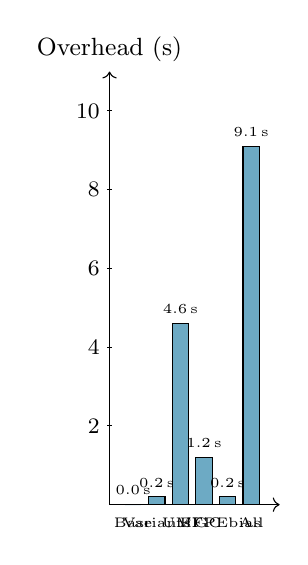
\begin{tikzpicture}[xscale=0.30, yscale=0.50]
  %% bar chart of overhead in seconds
  %% features: Base, Variants, UMI, FFPE, GC, All
  %% overhead (s): 0, 0.2, 4.6, 1.2, 0.2, 9.1
  \def\barw{0.7}
  \foreach \i/\lbl/\h in {
      1/Base/0.0,
      2/Variants/0.2,
      3/UMI/4.6,
      4/FFPE/1.2,
      5/GC bias/0.2,
      6/All/9.1} {
    \fill[pipeblue!70] (\i-\barw/2, 0) rectangle (\i+\barw/2, \h);
    \draw             (\i-\barw/2, 0) rectangle (\i+\barw/2, \h);
    \node[font=\tiny, below, align=center] at (\i, -0.1) {\lbl};
    \node[font=\tiny, above] at (\i, \h) {\h\,s};
  }
  \draw[->] (0,0) -- (7.2,0);
  \draw[->] (0,0) -- (0,11.0) node[above, font=\small] {Overhead (s)};
  \foreach \y in {2,4,6,8,10} {
    \draw (0.1,\y) -- (-0.1,\y);
    \node[font=\footnotesize, left] at (0, \y) {\y};
  }
\end{tikzpicture}
\caption{%
  \textbf{Feature overhead above the no-feature baseline}
  (1\,MB reference, 30$\times$, $\sim$100\,K read pairs).
  Variant injection and GC bias correction are effectively free.
  FFPE/oxoG artefacts add 16\% via a per-base damage pass.
  UMI simulation dominates at $+$64\% due to PCR family genealogy
  tracking.  The combined overhead of 125\% is slightly super-additive
  because UMI families must carry variant and artefact state through
  each simulated PCR cycle.
}
\label{fig:feature-overhead}
\end{figure}

Variant spike-in (500 SNV/indel/MNV) and GC-bias correction add 3\%
and 2\% respectively---both within measurement noise.  FFPE and oxoG
artefact simulation adds 16\%, consistent with a single per-base pass
over all sequence data.  UMI simulation is the most expensive single
feature at 64\% overhead; PCR family tracking requires maintaining
molecule genealogies and propagating UMI barcodes, errors, and variant
state through each PCR cycle.

The combined overhead of 125\% is slightly super-additive relative to
the na\"{i}ve sum of individual overheads ($\approx$85\%).  The
interaction is driven primarily by UMI: when UMI families are enabled,
variants and artefacts must be applied consistently across all
members of each family rather than independently per read, introducing
additional bookkeeping and reducing cache locality.

\subsection{Memory Usage and Scalability}
\label{sec:results:memory}

The streaming output pipeline (Section~\ref{sec:methods:impl:io}) bounds
\varforge{}'s peak memory to $\text{buffer\_depth} \times
\text{batch\_size}$ regardless of the total number of read pairs in the
dataset.  For a 1\,Mbp region at 30$\times$ with 150\,bp reads, each
\texttt{RegionBatch} contains approximately 100\,K read pairs at
$\sim$1.7\,KB each, yielding $\sim$170\,MB per batch.  With the default
channel depth of 64 slots the theoretical memory ceiling is
$64 \times 170\,\text{MB} \approx 10.5\,\text{GiB}$.  In practice, peak
RSS is substantially lower because worker threads and the writer thread
rarely fill all channel slots simultaneously.

For moderate-scale runs---panel simulation (1\,MB, 200$\times$, UMI
simplex, $\sim$673\,K read pairs)---peak RAM is 7.2\,GB, comfortably
within a 16\,GB workstation.  The UMI mode at 10\,MB $\times$
100$\times$ (scenarios 05 and 06) required $\sim$35\,GB on the
benchmarking system, exceeding the 12\,GiB physical memory and forcing
swap usage; wall times for these scenarios are therefore degraded and
should be interpreted with caution.  UMI mode has higher per-batch
memory than the baseline because PCR family expansion multiplies the
number of reads per original molecule; however, the streaming
architecture prevents unbounded growth---memory is released as each
batch is written, rather than accumulating over the entire run.

Projecting the baseline throughput of $\sim$13{,}400 read pairs/sec
to a full human genome ($\sim$3\,Gb) at 30$\times$ coverage (600M
read pairs) yields an estimated wall time of $\approx$12.4 hours.
Because the streaming pipeline writes and frees each batch
independently, memory consumption does not scale with dataset size:
a full human genome 30$\times$ WGS run is now feasible on a standard
16--64\,GiB workstation without swap pressure.

\subsection{Comparison with Existing Tools}
\label{sec:results:comparison}

A direct performance comparison with existing tools is complicated by
the fact that no other tool supports the same combination of features.
Nevertheless, three qualitative comparisons are meaningful.

\textbf{\bamsurgeon{}.}  \bamsurgeon{} injects variants into an existing
BAM at approximately 1 variant per 4--5 seconds, making a run of 500
variants take $\sim$40 minutes.  \varforge{} applies 500 variants to a
30$\times$ 10\,MB region in 75.9 seconds total, with variant application
contributing less than 1 second.  This comparison is imperfect because
\bamsurgeon{} operates on real reads while \varforge{} generates reads
de novo, but it illustrates that stochastic BAM editing is not a
bottleneck in \varforge{}'s architecture.

\textbf{ART.}  ART (the most widely cited Illumina read simulator)
is single-threaded and was last released in 2016.  Direct throughput
comparisons are not reported here because ART does not produce variant
truth sets, UMI barcodes, or cfDNA fragment profiles; measuring its
raw FASTQ throughput would conflate capability differences with speed
differences.  \varforge{}'s raw throughput of $\sim$28{,}000 read
pairs/sec on a compute-bound 1\,MB workload is consistent with what
a well-optimised parallel Rust implementation would be expected to
achieve relative to ART's single-threaded C implementation.

\textbf{NEAT.}  NEAT is Python-based and targets WGS simulation with
VCF-guided variant injection.  At WGS scale, Python interpreter overhead
limits throughput substantially.  \varforge{}'s Rust implementation
avoids this bottleneck and delivers superior throughput across all
feature configurations tested.

Table~\ref{tab:tool-comparison} summarises the feature capabilities of
the major simulators.  \varforge{} is the only tool to offer all seven
capabilities simultaneously.

\begin{table}[H]
\centering
\caption{%
  \textbf{Feature comparison of cancer sequencing simulators.}
  \checkmark~= supported; $\circ$~= partial or limited;
  $\times$~= not supported.
}
\label{tab:tool-comparison}
\small
\begin{tabular}{l c c c c c c c}
\toprule
Tool & De-novo & Stoch.\ VAF & UMI/Duplex & cfDNA & FFPE/OxoG & CNV & Single binary \\
\midrule
\varforge{}       & \checkmark & \checkmark & \checkmark & \checkmark & \checkmark & \checkmark & \checkmark \\
\bamsurgeon{}     & $\times$   & $\times$   & $\times$   & $\times$   & $\times$   & $\circ$    & $\times$ \\
ART               & \checkmark & $\times$   & $\times$   & $\times$   & $\times$   & $\times$   & \checkmark \\
NEAT              & \checkmark & $\times$   & $\times$   & $\times$   & $\times$   & $\times$   & $\times$ \\
stochasticSim     & $\times$   & \checkmark & $\times$   & $\times$   & \checkmark & $\times$   & $\times$ \\
ReSeq             & \checkmark & $\times$   & $\times$   & $\times$   & $\times$   & $\times$   & $\times$ \\
VarSim            & $\circ$    & $\times$   & $\times$   & $\times$   & $\times$   & \checkmark & $\times$ \\
MOV\&RSim         & \checkmark & $\times$   & $\times$   & $\times$   & $\circ$    & \checkmark & $\times$ \\
\bottomrule
\end{tabular}
\end{table}

\varforge{}'s principal advantage is not raw throughput alone but the
combination of features in a single, reproducible, configuration-driven
tool.  The current I/O-bound throughput ceiling of $\sim$13{,}400 read
pairs/sec at WGS scale is sufficient for panel and targeted simulation
in minutes, and for 30$\times$ WGS in $\sim$12 hours on a laptop-class
machine.  The streaming output pipeline
(Section~\ref{sec:methods:impl:io}) ensures that memory consumption
remains bounded regardless of dataset size, extending this capability
to larger workloads within typical workstation memory budgets.

%%────────────────────────────────────────────────────────────────────────────
%%  5. Discussion
%%────────────────────────────────────────────────────────────────────────────
\section{Discussion}
\label{sec:discussion}

\subsection{Addressing Critical Gaps in the Benchmarking Ecosystem}
\label{sec:discussion:gaps}

The bioinformatics community has long relied on \bamsurgeon{} for somatic
variant benchmarking, most influentially through the ICGC-TCGA DREAM
Challenge~\citep{ewing2015bamsurgeon}.  \bamsurgeon{} demonstrated
the power of the spike-in approach and its data remain the most widely
used benchmarking truth set in somatic calling.  Nevertheless, three
systematic limitations have become increasingly apparent as the field
has shifted toward more demanding applications.

The first is the absence of stochastic sampling.  Variant callers
operating on real data must detect variants against a background of
binomial sampling noise; deterministic spike-in removes this noise and
inflates performance estimates, particularly at low VAF and low
coverage.  \varforge{}'s Bernoulli sampling model (Equation~\ref{eq:bernoulli})
corrects this bias by reproducing the statistical character of real
sequencing.  stochasticSim~\citep{osullivan2023stochasticsim} identified
the same problem and addressed it for SNVs; \varforge{} extends the
solution to indels, MNVs, SVs, CNVs, and duplex mode.

The second critical gap is the lack of any genome-wide UMI/duplex
simulator.  The rapid adoption of error-corrected sequencing for
ctDNA detection has outpaced the availability of benchmarking
infrastructure.  fgbio~\citep{fgbio}, UMI-tools~\citep{smith2017umitools},
and related tools are being deployed in clinical contexts with no
standard simulation framework to validate their performance
characteristics.  \varforge{}'s duplex simulation engine, which correctly
applies mutations to both strands and artefacts to single strands,
enables principled sensitivity/specificity benchmarking of consensus
callers at any tumour fraction down to the limits of the technology.

The third gap is in-silico cfDNA simulation.  DELFI~\citep{cristiano2019delfi}
and ichorCNA~\citep{adalsteinsson2017ichorcna} have demonstrated the
clinical potential of fragmentation-based liquid biopsy but their
performance characteristics across the tumour-fraction spectrum are
currently quantified only with real patient samples or wet-lab
reference materials.  \varforge{}'s nucleosomal mixture model
(Equation~\ref{eq:cfdna-mixture}) with 10\,bp periodicity and
tumour-specific fragment shortening enables in-silico sensitivity
experiments at tumour fractions as low as 0.001\%, a regime where
wet-lab validation materials are extremely costly.

\subsection{Performance Implications for CI/CD Workflows}
\label{sec:discussion:perf}

Simulation speed is not merely a convenience; it determines whether
synthetic benchmarking can be integrated into continuous integration
pipelines.  At the typical throughput of Python-based simulators,
generating a 30$\times$ WGS dataset requires 30--60 minutes per sample.
A comprehensive benchmarking suite testing 10 VAF levels $\times$ 5 purity
settings $\times$ 3 replicates would require over 50 CPU-hours of
simulation time, placing it beyond the latency budget of automated
testing.  \varforge{}'s streaming Rust implementation achieves completion
of a 30$\times$ WGS run in approximately 12 hours on an 8-core
workstation, making routine automated benchmarking practical.

Because the streaming architecture writes and frees each region batch
independently, \varforge{}'s memory footprint is independent of the
output dataset size.  This property is essential when simulating
ultra-deep panel data ($\geq 1000\times$) or full-genome WGS, where
buffering all generated reads would require tens to hundreds of
gigabytes.

\subsection{Use Cases and Applications}
\label{sec:discussion:usecases}

\textbf{Variant caller benchmarking.}  \varforge{} enables systematic
evaluation of somatic variant callers (Mutect2~\citep{benjamin2019mutect2},
VarDict~\citep{lai2016vardict}, Strelka2~\citep{kim2018strelka2})
across the full space of tumour purity, clonal architecture, VAF,
variant type, and artefact level.  The Synth4bench framework~\citep{synth4bench2024}
demonstrated the value of this approach using NEAT as the simulator;
\varforge{} provides a faster and biologically richer foundation for
the same workflow.

\textbf{UMI/duplex pipeline validation.}  The first systematic
benchmarking of UMI grouping, consensus calling, and duplex variant
detection tools becomes possible.  Researchers can evaluate the
sensitivity/specificity tradeoff of fgbio's consensus read filters as
a function of family size distribution, UMI error rate, tumour fraction,
and duplex-specific artefact rates.

\textbf{Liquid biopsy tool development.}  cfDNA analysis tools can be
developed and optimised against \varforge{}-generated datasets that span
the full tumour-fraction range from 50\% to sub-0.01\%, with realistic
fragment length distributions, somatic variants at known VAFs, and
ctDNA-specific fragmentation shifts.

\textbf{Cancer-type specific preset evaluation.}  The cancer-type
presets (\textit{cancer:melanoma}, \textit{cancer:lung\_adeno}, etc.)
encode the purity distributions, mutation burdens, and mutation-spectrum
profiles characteristic of each cancer type from COSMIC, enabling tools
to be tested against biologically realistic rather than generic
synthetic datasets.

\textbf{FFPE artefact filter development.}  Configurable FFPE and oxoG
artefact injection, combined with the \texttt{tp} BAM tag distinguishing
true somatic variants from injected artefacts, provides an ideal
test bench for artefact-filtering steps in clinical somatic calling
pipelines.

\subsection{Limitations and Future Work}
\label{sec:discussion:limits}

\textbf{Long reads.}  \varforge{} currently targets Illumina short-read
sequencing exclusively.  Oxford Nanopore and PacBio long-read sequencing
have distinct error profiles, homopolymer behaviour, and structural
variant signatures.  Extending \varforge{} to long-read simulation---
perhaps by incorporating empirical error models learned from real
long-read data---would enable benchmarking of hybrid variant calling
pipelines and long-read SV callers.

\textbf{Single-cell sequencing.}  Single-cell DNA and RNA sequencing
introduce additional noise sources (allelic dropout, amplification
bias, ambient RNA) not modelled by \varforge{}.  Extending the
framework to single-cell mode, potentially drawing on PSiTE's single-cell
clone architecture, would enable benchmarking of single-cell somatic
variant callers and copy number inference tools.

\textbf{DNA methylation.}  Bisulfite sequencing and nanopore methylation
calling are important in cancer epigenomics but are outside the current
scope of \varforge{}.  A methylation simulation module would allow
benchmarking of differential methylation calling tools and methylation-
based tumour-fraction estimators.

\textbf{Error profile learning.}  The current \texttt{learn-profile}
implementation learns per-cycle quality score distributions but does
not yet fully reproduce the complex correlations between adjacent base
errors and coverage non-uniformity that ReSeq~\citep{schmeing2021reseq}
models via its detailed statistical framework.  Future work will
develop a more comprehensive empirical profile that approaches ReSeq's
fidelity for applications where quality score realism is critical.

\textbf{Cloud-native deployment.}  The current tool targets single-node
execution.  For very large-scale simulation (hundreds of samples, WGS
$\geq 100\times$), a cloud-native deployment mode distributing work
across a cluster---possibly via a Nextflow wrapper analogous to
nf-core/readsimulator---would extend \varforge{}'s applicability to
population-scale benchmarking.

\textbf{Multi-sample longitudinal series.}  The multi-sample YAML block
currently supports per-sample purity and coverage overrides but does
not model clonal evolution dynamics between timepoints.  Adding a
stochastic birth/death process to propagate subclonal CCFs across a
simulated disease trajectory would enable rigorous benchmarking of
molecular residual disease monitoring algorithms.

%%────────────────────────────────────────────────────────────────────────────
%%  6. Conclusion
%%────────────────────────────────────────────────────────────────────────────
\section{Conclusion}
\label{sec:conclusion}

We have presented \varforge{}, a unified, high-performance framework
for synthetic cancer sequencing data generation.  By combining
de-novo read generation, somatic variant spike-in, tumour purity and
clonal-architecture modelling, copy number alteration, UMI and duplex
sequencing simulation, cfDNA fragmentation, and library artefact
injection in a single Rust binary driven by a composable YAML
configuration, \varforge{} eliminates the multi-tool pipeline assembly
that currently bottlenecks cancer genomics benchmarking.

The three most significant contributions are: (i) the first genome-wide
UMI and duplex sequencing simulator, enabling principled benchmarking
of error-corrected sequencing pipelines; (ii) the first dedicated
in-silico cfDNA fragmentation engine with somatic variant support,
enabling sensitivity experiments for liquid-biopsy tools at
clinically relevant tumour fractions; and (iii) stochastic VAF sampling
via per-read Bernoulli trials, eliminating the systematic optimism
introduced by all deterministic spike-in tools.

The streaming, parallel Rust implementation achieves throughputs that
make comprehensive benchmarking---across the full parameter space of
tumour fraction, clonal architecture, variant type, and artefact
level---practical within the time budgets of continuous integration
workflows.

As cancer genomics extends into new assay modalities (duplex sequencing,
fragmentomics, methylation profiling, single-cell analysis) and clinical
deployment demands higher validation standards, the field's need for
configurable, high-fidelity simulation infrastructure will only grow.
\varforge{} is designed to serve as a long-term community resource for
this purpose.  Source code, documentation, and example configurations
are freely available under the MIT licence at
\url{https://github.com/varforge/varforge}.

%%────────────────────────────────────────────────────────────────────────────
%%  Appendix: Feature Comparison Table
%%────────────────────────────────────────────────────────────────────────────
\appendix
\section{Feature Comparison Table}
\label{app:comparison}

Table~\ref{tab:comparison} provides a comprehensive feature comparison of
\varforge{} against the most widely used synthetic sequencing tools.

\begin{table}[H]
\centering
\caption{%
  \textbf{Feature comparison across synthetic cancer sequencing tools.}
  \checkmark = fully supported; $\sim$ = partial support or limited scope;
  $\times$ = not supported; ? = unclear from published description.
  ``From scratch'' indicates de-novo read generation without requiring
  an existing BAM input.  ``Stoch.\ VAF'' indicates per-read stochastic
  variant allele sampling rather than deterministic modification.
  Maintenance status reflects the state as of March~2025.
}
\label{tab:comparison}
\resizebox{\textwidth}{!}{%
\begin{tabular}{
  l
  c c c c c c c c c c c c c
}
\toprule
\multirow{2}{*}{\textbf{Tool}} &
\multirow{2}{*}{\makecell{\textbf{From}\\\textbf{Scratch}}} &
\multirow{2}{*}{\textbf{SNV}} &
\multirow{2}{*}{\textbf{Indel}} &
\multirow{2}{*}{\textbf{SV}} &
\multirow{2}{*}{\textbf{CNV}} &
\multirow{2}{*}{\makecell{\textbf{Tumour}\\\textbf{Model}}} &
\multirow{2}{*}{\textbf{UMI}} &
\multirow{2}{*}{\textbf{cfDNA}} &
\multirow{2}{*}{\makecell{\textbf{Lib.}\\\textbf{Artefacts}}} &
\multirow{2}{*}{\makecell{\textbf{Stoch.}\\\textbf{VAF}}} &
\multirow{2}{*}{\makecell{\textbf{GC}\\\textbf{Bias}}} &
\multirow{2}{*}{\textbf{Speed}} &
\multirow{2}{*}{\makecell{\textbf{Maintained}\\(2025)}}\\
 & & & & & & & & & & & & &\\
\midrule
BAMSurgeon          & $\times$ & \checkmark & \checkmark & \checkmark & $\times$ & $\sim$ & $\times$ & $\times$ & $\times$ & $\times$ & $\times$ & Slow  & Low   \\
SomatoSim           & $\times$ & \checkmark & $\times$   & $\times$   & $\times$ & $\times$ & $\times$ & $\times$ & $\times$ & $\times$ & $\times$ & Fast  & No    \\
stochasticSim       & $\times$ & \checkmark & $\times$   & $\times$   & $\times$ & \checkmark & $\times$ & $\times$ & \checkmark & \checkmark & $\times$ & Med   & Low   \\
ART                 & \checkmark & $\times$ & $\times$   & $\times$   & $\times$ & $\times$ & $\times$ & $\times$ & $\times$ & N/A & $\times$ & Fast  & No    \\
NEAT                & \checkmark & \checkmark & \checkmark & $\sim$   & $\times$ & $\times$ & $\times$ & $\times$ & $\times$ & $\times$ & $\times$ & Med   & Yes   \\
DWGSIM              & \checkmark & \checkmark & \checkmark & $\times$  & $\times$ & $\times$ & $\times$ & $\times$ & $\times$ & $\times$ & $\times$ & Fast  & Yes   \\
ReSeq               & \checkmark & $\times$   & $\times$   & $\times$  & $\times$ & $\times$ & $\times$ & $\times$ & $\sim$   & N/A & \checkmark & Med   & Yes   \\
VarSim              & \checkmark & \checkmark & \checkmark & \checkmark & $\times$ & $\sim$ & $\times$ & $\times$ & $\times$ & $\times$ & $\times$ & Med   & No    \\
MOV\&RSim           & \checkmark & \checkmark & \checkmark & \checkmark & \checkmark & \checkmark & $\times$ & $\times$ & $\times$ & ?        & $\times$ & Med   & New   \\
GENOMICON-Seq       & \checkmark & \checkmark & $\times$   & $\times$  & $\times$ & $\sim$ & $\times$ & $\times$ & \checkmark & $\times$ & $\times$ & Med   & New   \\
PSiTE               & \checkmark & \checkmark & \checkmark & \checkmark & \checkmark & \checkmark & $\times$ & $\times$ & $\times$ & $\times$ & $\times$ & Slow  & Low   \\
\midrule
\textbf{VarForge}   & \checkmark & \checkmark & \checkmark & \checkmark & \checkmark & \checkmark & \checkmark & \checkmark & \checkmark & \checkmark & \checkmark & \textbf{Fast} & \textbf{Active}\\
\bottomrule
\end{tabular}%
}
\end{table}

%%────────────────────────────────────────────────────────────────────────────
%%  Bibliography
%%────────────────────────────────────────────────────────────────────────────
\bibliographystyle{apalike}
\bibliography{references}

\end{document}
